\documentclass[10pt]{article}
\usepackage[letterpaper,top=.55in,bottom=.46in,left=1.24in,right=.43in]{geometry}
\usepackage{amsmath,amssymb,mathtools,enumitem,booktabs}
\usepackage{fontspec}
\setmainfont[
  Path=C:/Users/notso/Documents/Latex/Multi Textbook/Fonts/Kalam/,
  UprightFont=Kalam-Regular.ttf,
  BoldFont=Kalam-Bold.ttf,
  ItalicFont=Kalam-Regular.ttf,
  BoldItalicFont=Kalam-Bold.ttf,
  Scale=0.98
]{Kalam-Regular.ttf}
\usepackage[italic]{mathastext}
\usepackage{pgfplots}
\pgfplotsset{compat=1.18}
\usepackage{tikz}
\usepackage{xcolor}
\pagestyle{empty}
\setlength{\parindent}{0pt}
\setlength{\parskip}{2pt}
\setlength{\abovedisplayskip}{4pt}
\setlength{\belowdisplayskip}{4pt}
\setlength{\abovedisplayshortskip}{2pt}
\setlength{\belowdisplayshortskip}{2pt}
\setlist{nosep,leftmargin=1.45em}
\allowdisplaybreaks
\newcommand{\ex}[1]{\par\addvspace{6pt}\noindent\llap{\makebox[.62in][r]{\large\bfseries #1.\hspace{.12in}}}\ignorespaces}
\newcommand{\ans}[1]{\underline{#1}}
\newcommand{\vv}[1]{\left\langle #1\right\rangle}
\newcommand{\ii}{\mathbf i}\newcommand{\jj}{\mathbf j}\newcommand{\kk}{\mathbf k}
\newcommand{\cp}[6]{\begin{vmatrix}\ii&\jj&\kk\\#1&#2&#3\\#4&#5&#6\end{vmatrix}}
\pgfplotsset{every axis/.append style={width=.70\linewidth,height=5.6cm,xlabel={$x$},ylabel={$y$},zlabel={$z$},view={125}{25},grid=major,font=\scriptsize}}
\newcommand{\surf}[4]{\begin{center}\begin{tikzpicture}\begin{axis}[#1]\addplot3[surf,shader=interp,samples=19,samples y=19,opacity=.78] ({#2},{#3},{#4});\end{axis}\end{tikzpicture}\end{center}}
\newcommand{\curve}[4]{\begin{center}\begin{tikzpicture}\begin{axis}[#1]\addplot3[blue,thick,samples=180,samples y=0,variable=t] ({#2},{#3},{#4});\end{axis}\end{tikzpicture}\end{center}}
\newcommand{\sectionstart}[2]{%
  \clearpage\thispagestyle{empty}\vspace*{.01in}%
  \noindent
  \begin{minipage}[t]{.17\textwidth}
    \tikz[baseline=(n.base)]\node[draw,rounded corners=1.5pt,line width=.8pt,inner xsep=8pt,inner ysep=4pt] (n) {\Large\bfseries #1};
  \end{minipage}\hfill
  \begin{minipage}[t]{.54\textwidth}\centering
    {\LARGE\bfseries Chapter 13 HW}\\[-2pt]
    {\normalsize #2}
  \end{minipage}\hfill
  \begin{minipage}[t]{.23\textwidth}\raggedleft
    {\large Anish Kumar}\\[-2pt]{\normalsize MW 6--8:35}
  \end{minipage}
  \par\vspace{.16in}%
}
\begin{document}
\small
\sectionstart{13.1}{Vector Functions and Space Curves}
\ex{1}
$r(t)=\vv{\ln(t+1),t/\sqrt{9-t^2},2^t}$. The logarithm requires $t+1>0$, or $t>-1$. The square root is in a denominator, so $9-t^2>0$, or $-3<t<3$. The exponential allows all real $t$. Intersect the restrictions: $\ans{(-1,3)}$.
\ex{5}
Take the limit of each component as $t\to\infty$:
\[\frac{1+t^2}{1-t^2}=\frac{t^{-2}+1}{t^{-2}-1}\to-1,\quad \tan^{-1}t\to\pi/2,\quad \frac{1-e^{-2t}}t\to0.\]
Thus $\ans{\lim r(t)=\vv{-1,\pi/2,0}}$.
\ex{11}
$x=t$, $y=2-t$, $z=2t$ describe the line $r=\vv{0,2,0}+t\vv{1,-1,2}$. As $t$ increases, $x,z$ increase and $y$ decreases. For example $t=0$ gives $(0,2,0)$ and $t=1$ gives $(1,1,2)$.
\begin{center}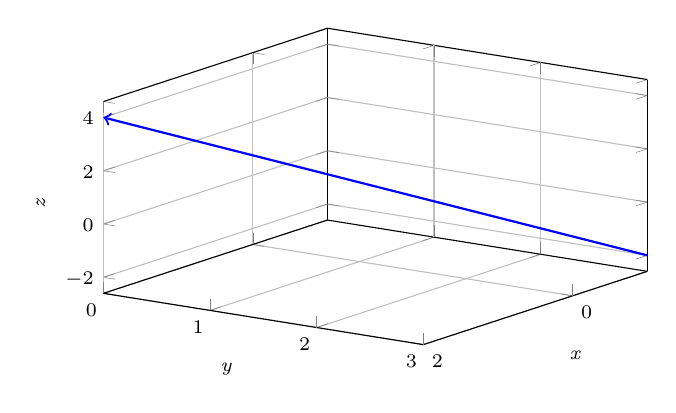
\begin{tikzpicture}\begin{axis}\addplot3[blue,thick,->] coordinates {(-1,3,-2)(2,0,4)};\end{axis}\end{tikzpicture}\end{center}
\ex{17}
Projection onto the $yz$-plane sets $x=0$ and preserves $y,z$: $r_{yz}(t)=\vv{0,t^3,t^{-3}}$, $t\ne0$. Eliminating $t$, $yz=t^3t^{-3}=1$, so $\ans{x=0,\ yz=1}$, a hyperbola with one branch in $y,z>0$ and another in $y,z<0$.
\begin{center}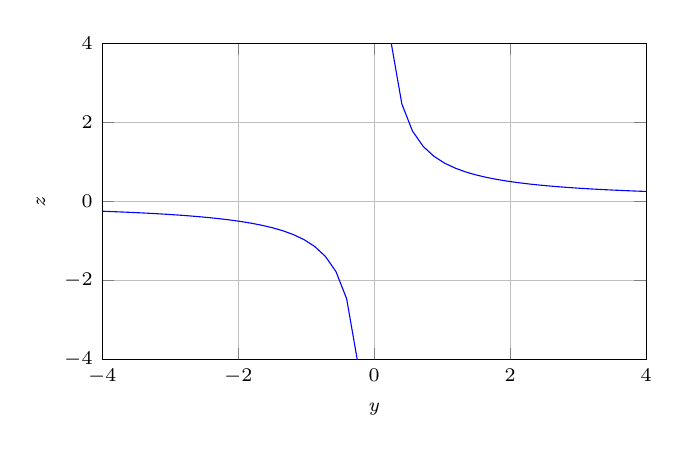
\begin{tikzpicture}\begin{axis}[view={0}{90},xlabel={$y$},ylabel={$z$},xmin=-4,xmax=4,ymin=-4,ymax=4]\addplot[blue,domain=.25:4]{1/x};\addplot[blue,domain=-4:-.25]{1/x};\end{axis}\end{tikzpicture}\end{center}
\ex{31}
$r(t)=\vv{t,4,t^2}$ has $y=4$ for every $t$, so the containing plane is $\ans{y=4}$. Within it the curve is $z=x^2$.
\ex{42}
$r(t)=\vv{te^t,e^{-t},t}$ is defined for all real $t$. Since $z=t$, eliminate the parameter: $x=ze^z$, $y=e^{-z}$. In particular $xy=z$, and $y>0$. As $t$ increases, height increases monotonically and $y$ decreases. The portion $-3\le t\le2$ displays the negative-$x$ bend and rapid positive-$x$ growth; $x'=e^t(1+t)$ changes sign at $t=-1$.
\curve{domain=-3:2}{t*exp(t)}{exp(-t)}{t}
\ex{43}
$r(t)=\vv{\sin3t\cos t,t/4,\sin3t\sin t}$. In cylindrical coordinates about $y$, the signed radius is $\sin3t$ and polar angle is $t$; $x^2+z^2=\sin^23t$. Thus it repeatedly expands to radius $1$ and contracts to the $y$-axis, while $y=t/4$ increases. Axis crossings occur at $t=n\pi/3$. The plot over $0\le t\le4\pi$ shows repeated lobes.
\curve{domain=0:12.56637}{sin(deg(3*t))*cos(deg(t))}{t/4}{sin(deg(3*t))*sin(deg(t))}
\ex{45}
$r(t)=\vv{\cos2t,\cos3t,\cos4t}$ is bounded by $[-1,1]^3$. Its common period is $2\pi$, so plot $0\le t\le2\pi$. Also $z=2x^2-1$ by the double-angle identity, so the curve lies on a parabolic cylinder. Since $r(-t)=r(t)$, the full period retraces the set described over $0\le t\le\pi$.
\curve{domain=0:6.283185}{cos(deg(2*t))}{cos(deg(3*t))}{cos(deg(4*t))}
\sectionstart{13.2}{Derivatives and Integrals of Vector Functions}
\ex{3}
\textbf{(a)} $x=t-2$ implies $t=x+2$, so $y=t^2+1=(x+2)^2+1$, a parabola with vertex $(-2,1)$.
\textbf{(b)} Differentiate componentwise: $\ans{r'(t)=\vv{1,2t}}$.
\textbf{(c)} At $t=-1$, the position is $r(-1)=\vv{-3,2}$ and tangent vector $r'(-1)=\vv{1,-2}$. The position arrow starts at the origin; the tangent arrow starts at $(-3,2)$ and ends at $(-2,0)$.
\begin{center}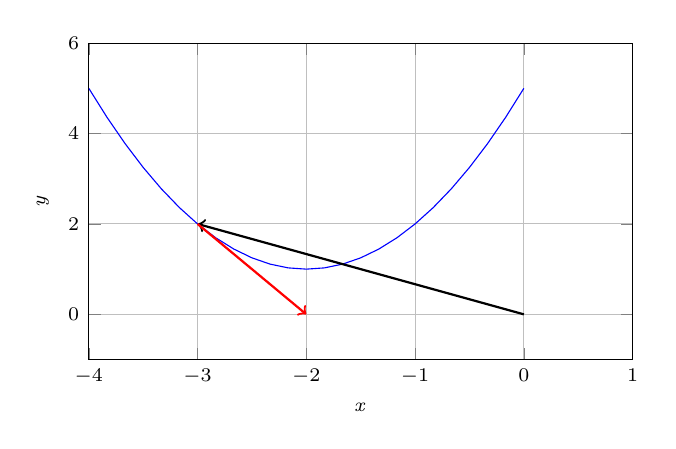
\begin{tikzpicture}\begin{axis}[view={0}{90},domain=-4:0,xmin=-4,xmax=1,ymin=-1,ymax=6]\addplot[blue]{(x+2)^2+1};\addplot[black,->,thick] coordinates {(0,0)(-3,2)};\addplot[red,->,thick] coordinates {(-3,2)(-2,0)};\end{axis}\end{tikzpicture}\end{center}
\ex{13}
Apply the product rule to the first two components and to $\sin t\cos t$:
\begin{align*}(t\sin t)'&=\sin t+t\cos t,\\(e^t\cos t)'&=e^t\cos t-e^t\sin t,\\(\sin t\cos t)'&=\cos^2t-\sin^2t=\cos2t.\end{align*}
Therefore $\ans{r'(t)=\vv{\sin t+t\cos t,e^t(\cos t-\sin t),\cos2t}}$.
\ex{15}
$a,b,c$ are constant vectors. Their derivatives are zero, so $\ans{(a+tb+t^2c)'=b+2tc}$.
\ex{17}
$r(t)=\vv{t^2-2t,1+3t,t^3/3+t^2/2}$. Hence $r'(t)=\vv{2t-2,3,t^2+t}$ and $r'(2)=\vv{2,3,6}$. Its length is $\sqrt{4+9+36}=7$, giving $\ans{T(2)=\vv{2,3,6}/7}$.
\ex{19}
$r(t)=\vv{\cos t,3t,2\sin2t}$ gives $r'(t)=\vv{-\sin t,3,4\cos2t}$. At zero, $r'(0)=\vv{0,3,4}$ has length $5$, so $\ans{T(0)=\vv{0,3/5,4/5}}$.
\ex{21}
At $(2,-2,4)$, the $y$ equation $3t-5=-2$ gives $t=1$; the other components also agree. Differentiate $r(t)=\vv{t^3+1,3t-5,4/t}$:
\[r'(t)=\vv{3t^2,3,-4/t^2},\quad r'(1)=\vv{3,3,-4},\quad|r'(1)|=\sqrt{34}.\]
Thus $\ans{T=\vv{3,3,-4}/\sqrt{34}}$.
\ex{25}
$y=4\sqrt t=4$ gives $t=1$, which also gives $x=2$, $z=1$. Differentiating,
\[r'(t)=\vv{2t,2/\sqrt t,(2t-1)e^{t^2-t}},\quad r'(1)=\vv{2,2,1}.\]
The tangent line uses an independent parameter $s$: $\ans{x=2+2s,\ y=4+2s,\ z=1+s}$.
\ex{27}
At $(1,0,1)$, $z=e^{-t}=1$ gives $t=0$. By the product rule,
\[r'(t)=\vv{-e^{-t}(\cos t+\sin t),e^{-t}(\cos t-\sin t),-e^{-t}}.\]
Thus $r'(0)=\vv{-1,1,-1}$ and the tangent line is $\ans{x=1-s,\ y=s,\ z=1-s}$.
\ex{35}
The origin corresponds to $t=0$ on both curves. Their tangent directions there are $r_1'(0)=\vv{1,0,0}$ and $r_2'(0)=\vv{1,2,1}$. Thus $\cos\theta=1/\sqrt6$, giving $\ans{\theta\approx66^\circ}$ to the nearest degree.
\ex{37}
Integrate each component from $0$ to $2$:
\[\int_0^2\vv{t,-t^3,3t^5}\,dt=\left[\vv{t^2/2,-t^4/4,t^6/2}\right]_0^2=\ans{\vv{2,-4,32}}.\]
\ex{39}
The three antiderivatives are $\ln(t+1)$, $\tan^{-1}t$, and $\tfrac12\ln(t^2+1)$ (using $u=t^2+1$ for the third). Evaluate from $0$ to $1$:
\[\ans{\vv{\ln2,\pi/4,(\ln2)/2}}.\]
\ex{41}
Integrate componentwise. For $te^{t^2}$ use $u=t^2$, $du=2t\,dt$:
\[\ans{\int\vv{(1+t^2)^{-1},te^{t^2},\sqrt t}\,dt=\vv{\tan^{-1}t,e^{t^2}/2,2t^{3/2}/3}+C}.\]
$C$ is an arbitrary constant vector, and the real integrand requires $t\ge0$.
\ex{51}
The dot-product rule is $f'=u'\cdot v+u\cdot v'$. At $2$, $v(2)=\vv{2,4,8}$ and $v'(2)=\vv{1,4,12}$. Therefore
\[f'(2)=\vv{3,0,4}\cdot\vv{2,4,8}+\vv{1,2,-1}\cdot\vv{1,4,12}=(6+0+32)+(1+8-12)=\ans{35}.\]
\sectionstart{13.3}{Arc Length and Curvature}
For a regular curve, $L=\int|r'|\,dt$, $T=r'/|r'|$, $N=T'/|T'|$, and $\kappa=|T'|/|r'|=|r'\times r''|/|r'|^3$.
\ex{1}
\textbf{(a)} $r'(t)=\vv{-1,2,4}$ has length $\sqrt{1+4+16}=\sqrt{21}$. Thus $L=\int_1^3\sqrt{21}\,dt=\ans{2\sqrt{21}}$.
\textbf{(b)} Endpoints are $r(1)=(2,2,5)$ and $r(3)=(0,6,13)$. Distance $\sqrt{(-2)^2+4^2+8^2}=\sqrt{84}=2\sqrt{21}$ agrees.
\ex{3}
$r'=\vv{1,-3\sin t,3\cos t}$. Speed is $\sqrt{1+9\sin^2t+9\cos^2t}=\sqrt{10}$. Hence $L=\int_{-5}^5\sqrt{10}\,dt=\ans{10\sqrt{10}}$.
\ex{5}
$r'=\vv{\sqrt2,e^t,-e^{-t}}$, so speed is
\[\sqrt{2+e^{2t}+e^{-2t}}=\sqrt{(e^t+e^{-t})^2}=e^t+e^{-t}.\]
Thus $L=\int_0^1(e^t+e^{-t})\,dt=[e^t-e^{-t}]_0^1=\ans{e-e^{-1}}$.
\ex{11}
The endpoints correspond to $t=0$ and $t=2$ because $y=2t$. With $r=\vv{\cos\pi t,2t,\sin2\pi t}$,
\[r'=\vv{-\pi\sin\pi t,2,2\pi\cos2\pi t},\quad L=\int_0^2\sqrt{\pi^2\sin^2\pi t+4+4\pi^2\cos^22\pi t}\,dt.\]
Numerical quadrature yields $\ans{L\approx 10.3311}$ (four decimal places).
\ex{15}
\textbf{(a)} $P=(4,1,3)$ corresponds to $t=1$. The direction $r'=\vv{-1,4,3}$ has length $\sqrt{26}$. Arc length from $P$ in the positive direction is $s=\sqrt{26}(t-1)$, so $t=1+s/\sqrt{26}$. Substitute:
\[\ans{r(s)=\vv{4-s/\sqrt{26},1+4s/\sqrt{26},3+3s/\sqrt{26}},\ s\ge0}.\]
\textbf{(b)} Four units along means $s=4$: $\ans{(4-4/\sqrt{26},1+16/\sqrt{26},3+12/\sqrt{26})}$.
\ex{17}
At $(0,0,3)$, $t=0$. For $r(t)=\vv{3\sin t,4t,3\cos t}$, speed $\sqrt{9\cos^2t+16+9\sin^2t}=5$. Thus $5=\int_0^t5\,du=5t$ implies $t=1$, and the point is $\ans{(3\sin1,4,3\cos1)}$.
\ex{19}
\textbf{(a)} Differentiate the components:
\[r'=\vv{2t,\sin t-(\cos t-t\sin t),-\sin t+(\sin t+t\cos t)}=t\vv{2,\sin t,\cos t}.\]
For $t>0$, $|r'|=\sqrt5t$, hence $T=\vv{2,\sin t,\cos t}/\sqrt5$. Then $T'=\vv{0,\cos t,-\sin t}/\sqrt5$ has length $1/\sqrt5$, so $\ans{N=\vv{0,\cos t,-\sin t}}$.
\textbf{(b)} $\ans{\kappa=(1/\sqrt5)/(\sqrt5t)=1/(5t)}$.
\ex{21}
\textbf{(a)} $r'=\vv{1,2t,0}$ has speed $q=\sqrt{1+4t^2}$, so $T=\vv{1,2t,0}/q$. Differentiate using $q'=4t/q$:
\[T'=\frac{\vv{0,2,0}}q-\frac{4t\vv{1,2t,0}}{q^3}=\frac{\vv{-4t,2,0}}{q^3}.\]
Its length is $2/q^2$, so $\ans{N=\vv{-2t,1,0}/q}$.
\textbf{(b)} $\ans{\kappa=2/(1+4t^2)^{3/2}}$.
\ex{25}
$r=\vv{t^3,0,t^2}$, $r'=\vv{3t^2,0,2t}$, $r''=\vv{6t,0,2}$.
\begin{align*}r'\times r''&=\cp{3t^2}{0}{2t}{6t}{0}{2}\\&=\ii(0-0)-\jj(6t^2-12t^2)+\kk(0-0)=\vv{0,6t^2,0}.\end{align*}
Thus $|r'\times r''|=6t^2$ and $|r'|=|t|\sqrt{9t^2+4}$, giving $\ans{\kappa=6/(|t|(9t^2+4)^{3/2}),\ t\ne0}$. At $t=0$ the parametrization is not regular, so this curvature formula is undefined.
\ex{27}
$r'=\vv{2\sqrt6t,2,6t^2}$ and $r''=\vv{2\sqrt6,0,12t}$.
\begin{align*}r'\times r''&=\cp{2\sqrt6t}{2}{6t^2}{2\sqrt6}{0}{12t}\\&=\ii(24t-0)-\jj(24\sqrt6t^2-12\sqrt6t^2)+\kk(0-4\sqrt6)\\&=\vv{24t,-12\sqrt6t^2,-4\sqrt6}.\end{align*}
Its squared length is $576t^2+864t^4+96=96(1+3t^2)^2$. Meanwhile $|r'|^2=24t^2+4+36t^4=4(1+3t^2)^2$. Therefore
\[\ans{\kappa=\frac{4\sqrt6(1+3t^2)}{8(1+3t^2)^3}=\frac{\sqrt6}{2(1+3t^2)^2}}.\]
\ex{31}
For $y=x^4$, $y'=4x^3$ and $y''=12x^2$. The graph curvature formula gives $\ans{\kappa(x)=12x^2/(1+16x^6)^{3/2}}$.
\ex{37}
\textbf{(a)} The curve bends more tightly at $P$ than at $Q$, so $\ans{\kappa(P)>\kappa(Q)}$. Curvature measures turning per unit distance, not height.
\textbf{(b)} Sketch an osculating circle below the local maximum at $P$ and above the local minimum at $Q$, tangent at the marked point. A rough reading of the textbook's unit scale gives radii on the order of $R_P\approx0.8$--$1$ and $R_Q\approx2$--$3$, hence $\kappa(P)\approx1$--$1.3$ and $\kappa(Q)\approx0.3$--$0.5$. These are visual estimates, not exact values: no equation or precise coordinates are supplied.
\begin{center}\begin{tikzpicture}[scale=1.15]\draw[->](-1,0)--(6,0) node[right]{$x$};\draw[->](0,-.2)--(0,3.5) node[above]{$y$};\draw[blue](-.4,1.6) to[out=-35,in=180](0,1.5) to[out=0,in=180](1.4,2.4) to[out=0,in=180](4,.2) to[out=0,in=-95](5.5,2.4);\draw[red,dashed](1.4,1.5) circle(.9);\draw[orange,dashed](4,2.5) circle(2.3);\fill(1.4,2.4) circle(1.5pt) node[above]{$P$};\fill(4,.2) circle(1.5pt) node[below]{$Q$};\end{tikzpicture}\end{center}
\sectionstart{13.4}{Motion in Space: Velocity and Acceleration}
Use $v=r'$, $a=r''$, and speed $|v|$. For acceleration components, $a_T=(v\cdot a)/|v|$ and $a_N=|v\times a|/|v|$.
\ex{3}
$r=\vv{-t^2/2,t}$ gives $\ans{v=\vv{-t,1},\ a=\vv{-1,0},\ |v|=\sqrt{t^2+1}}$. At $t=2$, $r=(-2,2)$, $v=\vv{-2,1}$, $a=\vv{-1,0}$, speed $\sqrt5$. Eliminate $t=y$: $x=-y^2/2$, a left-opening parabola.
\begin{center}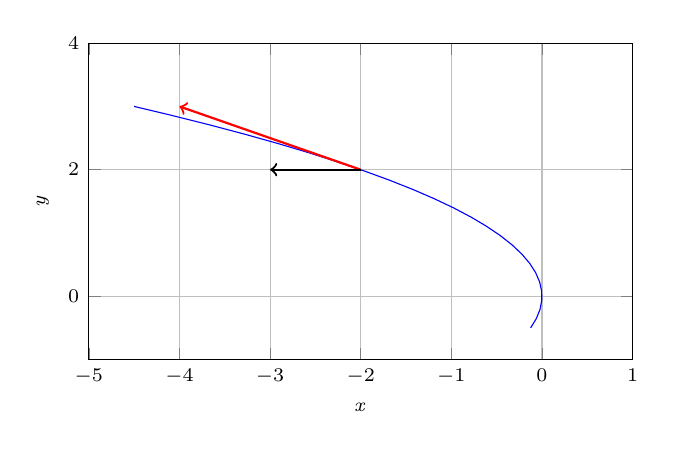
\begin{tikzpicture}\begin{axis}[view={0}{90},xmin=-5,xmax=1,ymin=-1,ymax=4]\addplot[blue,domain=-.5:3,variable=t] ({-t^2/2},{t});\addplot[red,thick,->] coordinates {(-2,2)(-4,3)};\addplot[black,thick,->] coordinates {(-2,2)(-3,2)};\end{axis}\end{tikzpicture}\end{center}
\ex{5}
$r=\vv{3\cos t,2\sin t}$ traces $x^2/9+y^2/4=1$ counterclockwise. Differentiate twice:
\[\ans{v=\vv{-3\sin t,2\cos t}},\quad\ans{a=\vv{-3\cos t,-2\sin t}},\quad\ans{|v|=\sqrt{9\sin^2t+4\cos^2t}}.\]
At $t=\pi/3$, $r=(3/2,\sqrt3)$, $v=\vv{-3\sqrt3/2,1}$, $a=\vv{-3/2,-\sqrt3}$, speed $\sqrt{31}/2$.
\begin{center}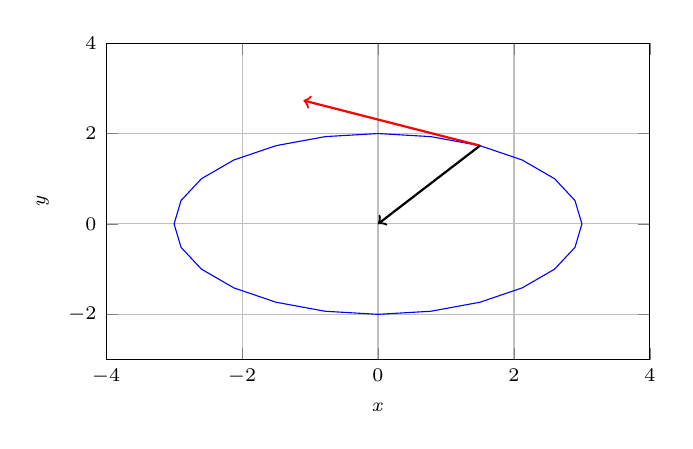
\begin{tikzpicture}\begin{axis}[view={0}{90},xmin=-4,xmax=4,ymin=-3,ymax=4]\addplot[blue,domain=0:360,variable=t] ({3*cos(t)},{2*sin(t)});\addplot[red,->,thick] coordinates {(1.5,1.732)(-1.098,2.732)};\addplot[black,->,thick] coordinates {(1.5,1.732)(0,0)};\end{axis}\end{tikzpicture}\end{center}
\ex{7}
$r=\vv{t,t^2,2}$ gives $\ans{v=\vv{1,2t,0},\ a=\vv{0,2,0},\ |v|=\sqrt{1+4t^2}}$. At $t=1$, $r=(1,1,2)$, $v=\vv{1,2,0}$, $a=\vv{0,2,0}$, speed $\sqrt5$. The path is the parabola $y=x^2$ in $z=2$.
\begin{center}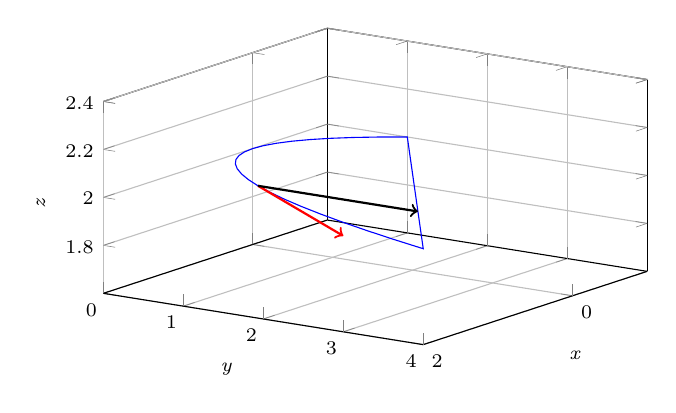
\begin{tikzpicture}\begin{axis}\addplot3[blue,domain=-1:2,variable=t]({t},{t^2},{2});\addplot3[red,->,thick]coordinates{(1,1,2)(2,3,2)};\addplot3[black,->,thick]coordinates{(1,1,2)(1,3,2)};\end{axis}\end{tikzpicture}\end{center}
\ex{9}
Differentiate each polynomial component:
\[\ans{v=\vv{2t+1,2t-1,3t^2}},\quad\ans{a=\vv{2,2,6t}}.\]
Speed $\sqrt{(2t+1)^2+(2t-1)^2+9t^4}=\ans{\sqrt{9t^4+8t^2+2}}$.
\ex{11}
$r=\vv{\sqrt2t,e^t,e^{-t}}$ gives $\ans{v=\vv{\sqrt2,e^t,-e^{-t}},\ a=\vv{0,e^t,e^{-t}}}$. Speed $\sqrt{2+e^{2t}+e^{-2t}}=\ans{e^t+e^{-t}}$.
\ex{13}
Apply the product rule to $e^t\vv{\cos t,\sin t,t}$:
\[\ans{v=e^t\vv{\cos t-\sin t,\sin t+\cos t,t+1}}.\]
A second derivative gives $\ans{a=e^t\vv{-2\sin t,2\cos t,t+2}}$. Since $(\cos t-\sin t)^2+(\sin t+\cos t)^2=2$, speed is $\ans{e^t\sqrt{2+(t+1)^2}}$.
\ex{15}
Integrate each component of $a=\vv{2,0,2t}$:
\[v=\vv{2t+C_1,C_2,t^2+C_3}.\]
Initial velocity $\vv{3,-1,0}$ gives $C_1=3$, $C_2=-1$, and $C_3=0$. Thus
\[\ans{v=\vv{2t+3,-1,t^2}}.\]
Integrate again:
\[r=\vv{t^2+3t+D_1,-t+D_2,t^3/3+D_3}.\]
Using $r(0)=\vv{0,1,1}$ gives $D_1=0$, $D_2=1$, and $D_3=1$, so
\[\ans{r=\vv{t^2+3t,1-t,1+t^3/3}}.\]
\ex{19}
$v=\vv{2t,5,2t-16}$, so speed squared is
\[4t^2+25+(2t-16)^2=8t^2-64t+281=8(t-4)^2+153.\]
This is minimized at $\ans{t=4}$ (and the minimum speed is $\sqrt{153}=3\sqrt{17}$). Minimizing speed squared is equivalent to minimizing nonnegative speed.
\ex{23}
Assume launch and landing at ground level, no air resistance, $g=9.8\ \mathrm{m/s^2}$. Horizontal velocity is $200\cos60^\circ=100$; initial vertical velocity is $200\sin60^\circ=100\sqrt3$. Thus $x=100t$, $y=100\sqrt3t-4.9t^2$.
\begin{enumerate}[label=(\alph*)]
\item Set $y=0$ at positive time: $T=200\sqrt3/9.8$. Range $R=100T=\ans{20000\sqrt3/9.8\approx3534.80\ \mathrm m}$.
\item At the peak $v_y=100\sqrt3-9.8t=0$, so $t_p=100\sqrt3/9.8$. Then $H=(100\sqrt3)^2/(2\cdot9.8)=\ans{15000/9.8\approx1530.61\ \mathrm m}$.
\item At impact, $v=\vv{100,-100\sqrt3}$. Its length is $\sqrt{10000+30000}=\ans{200\ \mathrm{m/s}}$.
\end{enumerate}
\ex{27}
Using $g=32\ \mathrm{ft/s^2}$, the maximum height is $H=v_0^2\sin^236^\circ/(2g)$. Therefore $1600=v_0^2\sin^236^\circ/64$, so
\[\ans{v_0=\frac{\sqrt{1600\cdot64}}{\sin36^\circ}=\frac{320}{\sin36^\circ}\approx544.42\ \mathrm{ft/s}}.\]
\ex{37}
$r=\vv{t^2+1,t^3,0}$, $v=\vv{2t,3t^2,0}$, $a=\vv{2,6t,0}$. For $t>0$, $|v|=t\sqrt{4+9t^2}$ and $v\cdot a=4t+18t^3$, hence
\[\ans{a_T=\frac{4+18t^2}{\sqrt{4+9t^2}}}.\]
\[v\times a=\cp{2t}{3t^2}{0}{2}{6t}{0}=\ii(0)-\jj(0)+\kk(12t^2-6t^2)=\vv{0,0,6t^2}.\]
Thus $\ans{a_N=6t/\sqrt{4+9t^2}}$. At $t=0$, $v=0$ so the usual formulas are undefined; their one-sided limits are $a_T\to2$, $a_N\to0$.
\ex{39}
$v=\vv{-\sin t,\cos t,1}$, $a=\vv{-\cos t,-\sin t,0}$. Speed $\sqrt2$ is constant and $v\cdot a=\sin t\cos t-\cos t\sin t=0$, so $\ans{a_T=0}$. Since $|a|=1$ and $|a|^2=a_T^2+a_N^2$, $\ans{a_N=1}$.
\ex{41}
At $(0,4,4)$, $\ln t=0$ implies $t=1$; the other coordinates agree. For $r=\vv{\ln t,t^2+3t,4\sqrt t}$,
\[v=\vv{1/t,2t+3,2/\sqrt t},\quad a=\vv{-1/t^2,2,-t^{-3/2}}.\]
At $1$, $v=\vv{1,5,2}$, $a=\vv{-1,2,-1}$, $|v|=\sqrt{30}$, $v\cdot a=-1+10-2=7$. Thus $\ans{a_T=7/\sqrt{30}}$.
\begin{align*}v\times a&=\cp{1}{5}{2}{-1}{2}{-1}\\&=\ii[5(-1)-2(2)]-\jj[1(-1)-2(-1)]+\kk[1(2)-5(-1)]\\&=\vv{-9,-1,7}.
\end{align*}
Its length is $\sqrt{81+1+49}=\sqrt{131}$, so $\ans{a_N=\sqrt{131/30}}$.
\end{document}
